% !TEX encoding = UTF-8 Unicode

% Based on https://github.com/Miracle0565/BUCT-Beamer-Theme

\documentclass[
10pt, 
aspectratio=43, 
]{beamer}
\setbeamercovered{transparent=10}
\usetheme[
%  showheader, 
%  red, 
  purple, 
%  gray, 
%  graytitle, 
  colorblocks, 
%  noframetitlerule, 
]{Verona}

\usepackage[T1]{fontenc}
\usepackage[utf8]{inputenc}
\usepackage{lipsum}
%%%%%%%%%%%%%%%%%%%%%%%%%%%%%%%
% Mac上使用如下命令声明隶书字体, windows也有相关方式, 大家可自行修改
\providecommand{\lishu}{\CJKfamily{zhli}}
%%%%%%%%%%%%%%%%%%%%%%%%%%%%%%%
\usepackage{tikz}
\usetikzlibrary{fadings}
%
%\setbeamertemplate{sections/subsections in toc}[ball]
\usepackage{xeCJK}
\usepackage{tikz}
\usepackage{listings}
\usepackage{caption}
\usepackage{subfigure}
\usefonttheme{professionalfonts}
\def\mathfamilydefault{\rmdefault}
\usepackage{amsmath}
\usepackage{multirow}
\usepackage{booktabs}
\usepackage{bm}
\setbeamertemplate{section in toc}{\hspace*{1em}\inserttocsectionnumber.~\inserttocsection\par}
\setbeamertemplate{subsection in toc}{\hspace*{2em}\inserttocsectionnumber.\inserttocsubsectionnumber.~\inserttocsubsection\par}
\setbeamerfont{subsection in toc}{size=\small}
\AtBeginSection[]{%
	\begin{frame}%
		\frametitle{Outline}%
		\textbf{\tableofcontents[currentsection]} %
	\end{frame}%
}

\AtBeginSubsection[]{%
	\begin{frame}%
		\frametitle{Outline}%
		\textbf{\tableofcontents[currentsection,  currentsubsection]} %
	\end{frame}%
}

\title{高等数学C}
%\subtitle{A Simple while elegant template}
\author[P.Yu]{余沛}
\mail{peiy\_gzgs@qq.com}
\institute[Guangzhou College of Technology and Business]{Guangzhou College of Technology and Business \\
  广州工商学院}
\date{\today}
\titlegraphic[width=4cm]{logo.png}{}




%%%%%%%%%%%%%%%%%%%%%%%%%%%%%%%%
% ----------- 标题页 ------------
%%%%%%%%%%%%%%%%%%%%%%%%%%%%%%%%



\begin{document}

\maketitle

%%% define code
\defverbatim[colored]\lstI{
	\begin{lstlisting}[language=C++, basicstyle=\ttfamily, keywordstyle=\color{red}]
	int main() {
	// Define variables at the beginning
	// of the block,  as in C: 
	CStash intStash,  stringStash;
	int i;
	char* cp;
	ifstream in;
	string line;
	[...]
	\end{lstlisting}
}
%%%%%%%%%%%%%%%%%%%%%%%%%%%%%%%%
% ----------- FRAME ------------
%%%%%%%%%%%%%%%%%%%%%%%%%%%%%%%%

\section{数列极限}
\subsection{割圆术与圆的周长求解}
\begin{frame}{割圆术与圆的周长求解}
	\begin{columns}
		\column{0.5\textwidth}
		\begin{figure}
			\centering
			% Requires \usepackage{graphicx}
			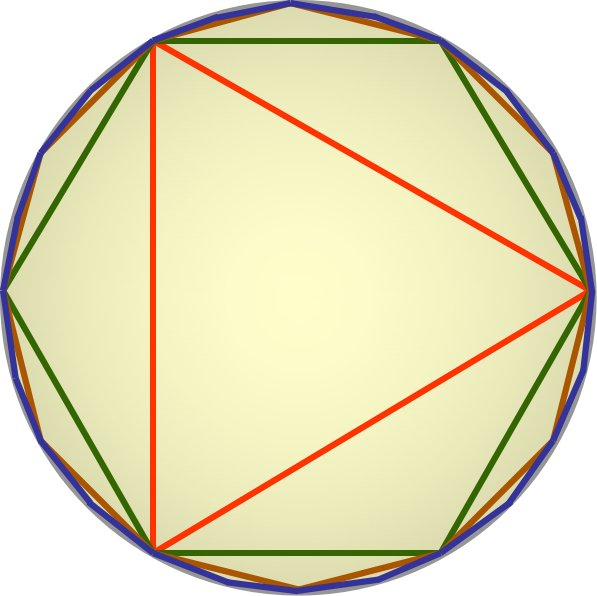
\includegraphics[width=5cm]{割圆术}
			\caption{割圆术示意图}
		\end{figure}
		\column{0.55\textwidth}
		\small
		\begin{itemize}	
			\item 刘徽(生平不详. 魏景元四年(263年)著有《九章算术注》10卷. )提出的方法.他把圆周分成三等分、六等分、十二等分、二十四等分... 这样继续分割下去, 所得多边形的周长就无限接近于圆的周长. \newline \newline
			\item 思路: 单调有界数列有极限. \newline \newline
			\item 第 $n$ 次等分所得到的的周长是多少? \newline \newline
			\item $\displaystyle 2n\times R\times \sin \frac{2\pi}{2n}$
		\end{itemize}
	\end{columns}
\end{frame}

\subsection{数列极限}
\subsubsection{数列的定义}
\begin{frame}{什么是数列}
	\begin{columns}
		\column{0.5\textwidth}
		\begin{block}{定义: 数列}
			数列是按照一定规律排列的一组数的集合, 其中每个数都有一个确定的位置, 称为索引或项号. 数列的一般形式可以表示为: 
			\begin{equation*}
				\{ a_1,  a_2,  a_3,  \ldots,  a_n,  \ldots \}, 
			\end{equation*}
		\end{block}
		定义: 数列是按照一定规律排列的一组数的集合, 其中每个数都有一个确定的位置, 称为索引或项号. 数列的一般形式可以表示为: 
		\begin{equation*}
			\{ a_1,  a_2,  a_3,  \ldots,  a_n,  \ldots \}, 
		\end{equation*}
		注意, 高等数学中体积的数列一般是具有无穷多项的. 
		\column{0.55\textwidth}
		\small
		一些例子: 
		\begin{equation*}
			\begin{array}{l}
				{\displaystyle\frac12, \frac23, \frac34, \ldots, \frac{n}{n+1}, \ldots;} \\
				{\displaystyle2, 4, 8, 16, \ldots, 2^n, \ldots;}                         \\
				{\displaystyle1, -1, 1, -1, \ldots, (-1)^{n+1}, \ldots;}                 \\
				{\displaystyle2, \frac12, \frac43, \ldots, \frac{n+(-1)^n}{n}, \ldots.}  
			\end{array}
		\end{equation*}
		如果能找到数列的一般项次的表达式, 就称之为通项公式. 这时候数列可以简单记为
		\begin{equation*}
			\{a_n\}\quad \text{或}\quad \{a_n\}_{n=1}^\infty.
		\end{equation*}
		以更直接地描述数列的性质. 
	\end{columns}
\end{frame}
\subsubsection{直观感受数列}
\begin{frame}{一些特例}
	\begin{columns}
		\column{0.5\textwidth}
		\begin{figure}
			\centering
			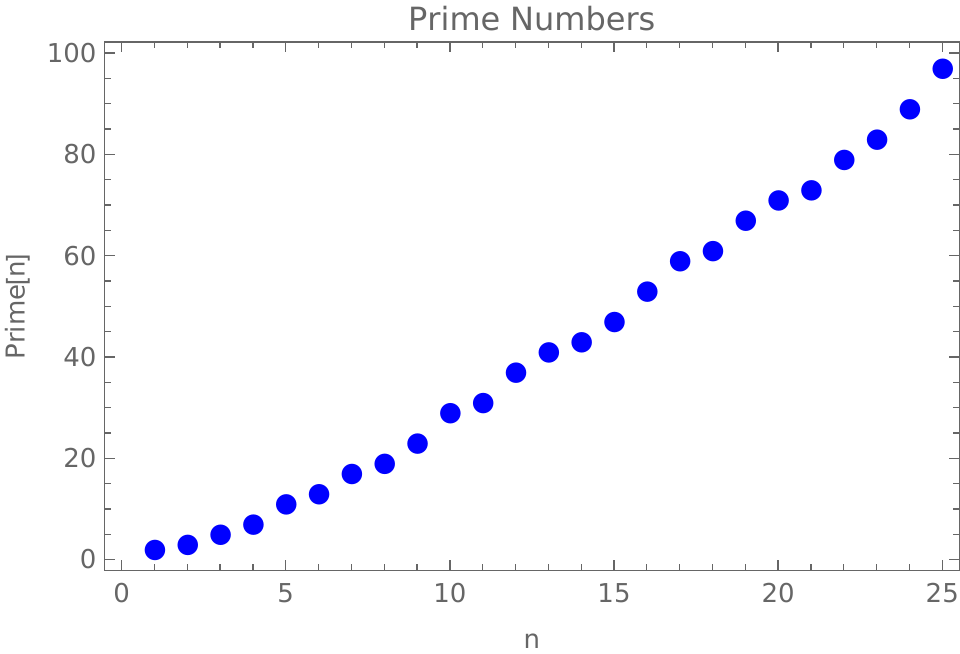
\includegraphics[width=0.8\linewidth]{prime.png}
			
		\end{figure}
		\begin{equation*}
			\begin{aligned}
				  & \pi(k)=                                                                                                                                    \\
				  & \sum_{j=2}^k\left[\frac{2}{j}\left(1+\sum_{s=1}^{[\sqrt{j}]}\left(\left[\frac{j-1}{s}\right]-\left[\frac{j}{s}\right]\right)\right)\right] \\
				  & +k+1                                                                                                                                       
			\end{aligned}
		\end{equation*}
		\column{0.55\textwidth}
		\small
		\begin{figure}
			\centering
			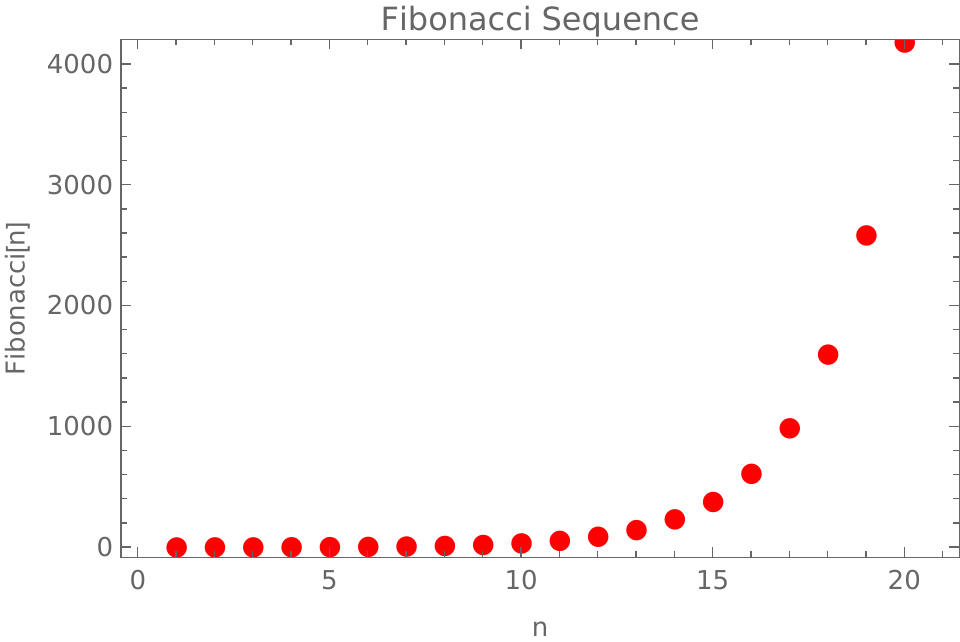
\includegraphics[width=0.8\linewidth]{fibonacci.png}
		\end{figure}
		\begin{equation*}
			F(n) = \frac{{(\frac{\sqrt{5}+1}{2})^n - (\frac{\sqrt{5}-1}{2})^{-n}}}{{\sqrt{5}}}.
		\end{equation*}
	\end{columns}
\end{frame}

\begin{frame}{动动手}
	
	\begin{itemize}
		\item 代码展示-数学软件: Matlab, \textcolor{blue}{Mathematica}, Maple, \textcolor{red}{GNU Octave},  ...\\
		              
		\item 代码生成-大语言模型: \textcolor{blue}{chatGPT},  \textcolor{red}{chatGLM},  Falcon, llama,  ... 
	\end{itemize}
	
\end{frame}

\begin{frame}{动动手}
	举例: 希望观察 $n^4 e^{-n}$ 数列. 
	\begin{columns}
		\column{0.5\textwidth}
		\begin{figure}
			\centering
			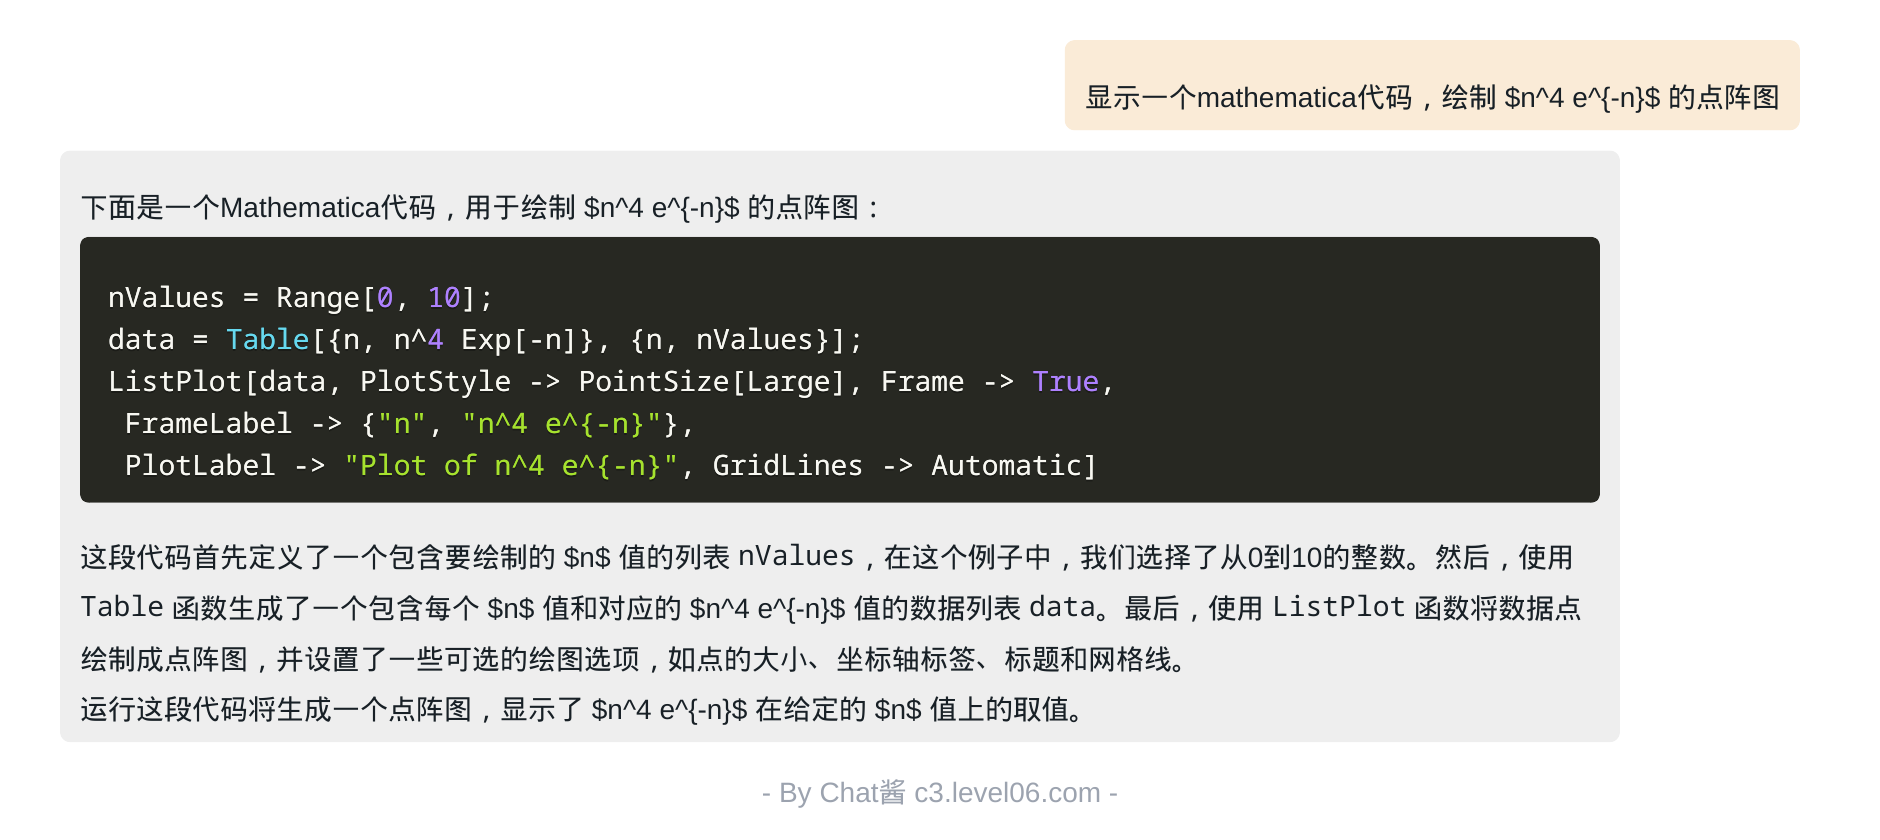
\includegraphics[width=1.2\linewidth]{Chat酱-1696676606183.png}
			\caption{对话}
			
		\end{figure}
		\column{0.55\textwidth}
		\small
		\begin{figure}
			\centering
			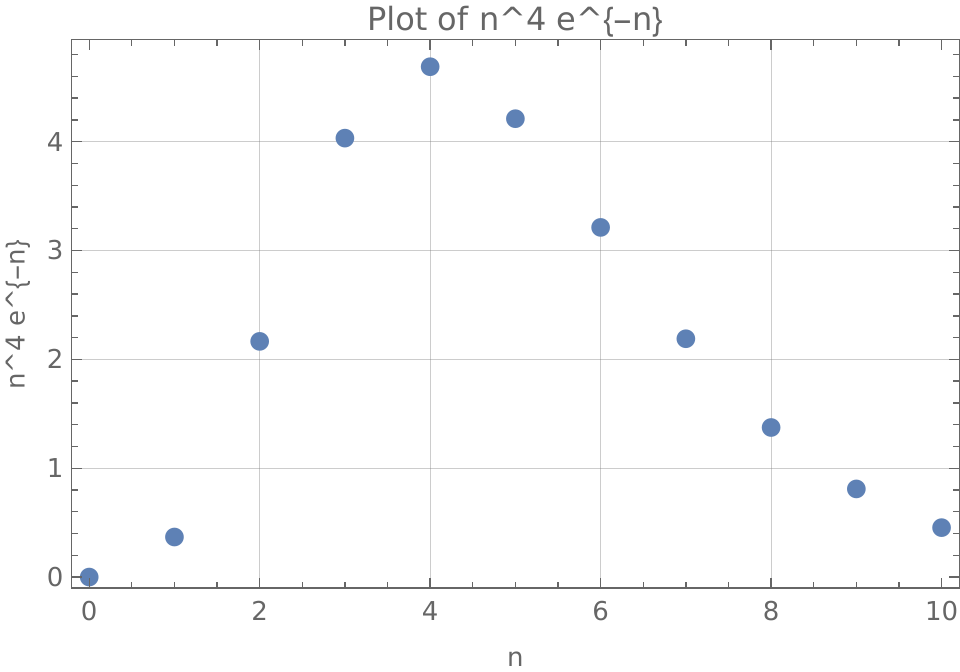
\includegraphics[width=0.8\linewidth]{n^4 Exp[-n].png}
			        
		\end{figure}
		\begin{equation}
			x_n = n^4 e^{-n}.
		\end{equation}
	\end{columns}
\end{frame}

\subsubsection{数列极限的定义}
\begin{frame}
	\begin{block}{定义: 数列极限与收敛数列}
		对于数列 $\{x_n\}$ 和常数 $a$, 如果有: 对于任意的 $\epsilon>0$, 都存在正整数 $N$, 使得对于任意满足 $n>N$ 的 $n$, 不等式
		$$|x_n-a|<\epsilon$$
		都成立, 
		那么称常数 $a$ 是数列 $\{x_n\}$ 的极限, 或者数列 $\{x_n\}$ 收敛, 并且收敛于 $a$, 记为
		\begin{equation*}
			\lim_{n\to\infty}x_n=a,  \quad \text{或} \quad x_n\to a (n\to\infty).
		\end{equation*}
	\end{block}
	\pause
	\begin{block}{发散数列}
		不收敛于任意常数a的数列. 
	\end{block}
	\pause
	\begin{exampleblock}{发散数列的确切定义是什么?}
		对于一个数列 ${a_n}$, 如果存在一个正实数 $\epsilon$, 对于任意的正整数 $N$, 都存在一个项数 $n>N$, 使得 $|a_n|>\epsilon$, 那么这个数列 ${a_n}$ 是发散的. 
	\end{exampleblock}
\end{frame}


\begin{frame}
	\frametitle{证明数列$n^{-1}\sin(n)$收敛到 0}
	
	为了证明数列 $n^{-1}\sin(n)$ 收敛到 0, 我们将使用数列收敛的定义. 
	
	\pause
	
	\begin{itemize}
		\item 设 $\epsilon > 0$, 我们需要找到一个正整数 $N$, 使得对于所有 $n \geq N$, 都有 $|n^{-1}\sin(n) - 0| < \epsilon$. 
		      
		      \pause
		      
		\item 由于对于所有 $n \in \mathbb{N}$, 有 $|\sin(n)| \leq 1$, 我们有 $|n^{-1}\sin(n)| \leq n^{-1}$. 
		      
		      \pause
		      
		\item 取 $N = \lceil \frac{1}{\epsilon} \rceil$. 对于所有 $n \geq N$, 我们有 $n^{-1} \leq \frac{1}{N} \leq \epsilon$. 
		      
		      
	\end{itemize}
	
	\pause
	
	因此, 对于所有 $n \geq N$, 我们有 $|n^{-1}\sin(n) - 0| = n^{-1}|\sin(n)| \leq n^{-1} \leq \epsilon$. 
	
	\pause
	
	根据数列收敛的定义, 数列 $n^{-1}\sin(n)$ 收敛到 0. 
	
\end{frame}

\begin{frame}
	\frametitle{证明数列 $x_n=\frac{n}{n+1}$ 收敛到1}
	我们要证明数列 $x_n=\frac{n}{n+1}$ 收敛到1. 
	\pause
	\textbf{证明: }
	对于任意给定的正实数 $\epsilon$, 我们需要找到一个正整数 $N$, 使得当 $n>N$ 时, $|x_n - 1| < \epsilon$. 
	\pause
	考虑 $|x_n - 1|$: 
	\[
		|x_n - 1| = \left|\frac{n}{n+1} - 1\right| = \left|\frac{n - (n+1)}{n+1}\right| = \left|\frac{-1}{n+1}\right| = \frac{1}{n+1}
	\]
	\pause
	为了使 $\frac{1}{n+1} < \epsilon$ 成立, 我们可以选择 $N = \frac{1}{\epsilon} - 1$. 
	\pause
	当 $n>N$ 时, 我们有: 
	\[
		\frac{1}{n+1} < \frac{1}{N+1} = \frac{1}{\frac{1}{\epsilon} - 1 + 1} = \epsilon
	\]
	\pause
	因此, 当 $n>N$ 时, $|x_n - 1| < \epsilon$. 
	\pause
	根据极限的定义, 我们可以得出结论: 数列 $x_n=\frac{n}{n+1}$ 收敛到1. 
\end{frame}

\subsection{数列极限的性质}

\begin{frame}
	\frametitle{收敛数列的性质}
	
	收敛数列是数学分析中的重要概念, 它具有以下性质: 
	
	\begin{enumerate}
		\item 收敛数列有唯一的极限. 
		      \pause
		\item 收敛数列的极限是有界的. 
		      \pause
		\item 收敛数列的子数列也收敛, 并且收敛于相同的极限. 
		      \pause
		\item 收敛数列的和、差、积仍然是收敛数列, 并且极限满足相应的运算规律. 
		      \pause
		\item 极限不为零收敛数列的倒数也是收敛数列, 且极限的倒数等于原数列极限的倒数. 
	\end{enumerate}
	
\end{frame}


\section{函数的极限}
\subsection{函数极限的定义}

\begin{frame}
	\frametitle{函数极限的数列定义}
	\begin{block}{函数极限的数列定义}
		设函数 $f(x)$ 在点 $x=a$ 的某个去心邻域内有定义, 如果存在常数 $L$, 对于任意定义在该去心邻域上收敛到$a$的数列 $\{x_n\}$, 都有 
		\begin{equation*}
			\lim_{n\to\infty} f(x_n) = L, 
		\end{equation*}
		则称函数 $f(x)$ 在 $x=a$ 处\textbf{收敛}于 $L$, 记作 $\lim_{x \to a} f(x) = L$. 
	\end{block}
	
	\pause
	
	\textbf{注意: }
	\begin{itemize}
		\item 函数极限的定义要求在去心邻域内有定义, 这是为了排除 $x=a$ 的情况. 
		      \pause
		\item 函数极限的定义要求对于任意给定的正实数 $\epsilon$, 都存在正实数 $\delta$, 使得当 $0 < |x-a| < \delta$ 时, $|f(x) - L| < \epsilon$ 成立. 这意味着无论 $\epsilon$ 有多小, 总存在一个足够小的 $\delta$, 使得函数值 $f(x)$ 与极限 $L$ 的差的绝对值小于 $\epsilon$. 
	\end{itemize}
	
\end{frame}

\begin{frame}
	\frametitle{函数极限的解析定义}
	\begin{block}{函数极限的解析定义}
		设函数 $f(x)$ 在点 $x=a$ 的某个去心邻域内有定义, 如果存在常数 $L$, 对于任意给定的正实数 $\epsilon$, 都存在正实数 $\delta$, 使得当 $0 < |x-a| < \delta$ 时, 有 $|f(x) - L| < \epsilon$ 成立, 则称函数 $f(x)$ 在 $x=a$ 处\textbf{收敛}于 $L$, 记作 $\lim_{x \to a} f(x) = L$. 
	\end{block}
\end{frame}


\begin{frame}
	\frametitle{函数极限的解析定义}
	
	设函数 $f(x)$ 在点 $x=a$ 的某个去心邻域内有定义, 如果存在常数 $L$, 对于任意给定的正实数 $\epsilon$, 都存在正实数 $\delta$, 使得当 $0 < |x-a| < \delta$ 时, 有 $|f(x) - L| < \epsilon$ 成立, 则称函数 $f(x)$ 在 $x=a$ 处\textbf{收敛}于 $L$, 记作 $\lim_{x \to a} f(x) = L$. 
	
	\pause
	
	\textbf{注意: }
	\begin{itemize}
		\item 函数极限的定义要求在去心邻域内有定义, 这是为了排除 $x=a$ 的情况. 
		      \pause
		\item 函数极限的定义要求对于任意给定的正实数 $\epsilon$, 都存在正实数 $\delta$, 使得当 $0 < |x-a| < \delta$ 时, $|f(x) - L| < \epsilon$ 成立. 这意味着无论 $\epsilon$ 有多小, 总存在一个足够小的 $\delta$, 使得函数值 $f(x)$ 与极限 $L$ 的差的绝对值小于 $\epsilon$. 
	\end{itemize}
	
\end{frame}

\begin{frame}
	\frametitle{$f(x) = x^2$ 在每一点都收敛}
	先来看 函数 $f(x) = x^2$
	\begin{center}
		\begin{tikzpicture}[scale=0.6]
			\draw[->] (-3, 0) -- (3, 0) node[right] {$x$};
			\draw[->] (0, -1) -- (0, 7) node[above] {$f(x)$};
			\draw[domain=-2.5: 2.5, smooth, variable=\x, blue] plot ({\x}, {\x*\x}) node[right] {$f(x) = x^2$};
		\end{tikzpicture}
	\end{center}
	
	函数 $f(x) = x^2$ 是一个抛物线, 开口朝上, 顶点位于原点. 
	
\end{frame}


\begin{frame}
	\frametitle{$f(x) = x^2$ 在每一点都收敛}
	
	考虑函数 $f(x) = x^2$. 
	
	\pause
	
	\textbf{定理: } 对于函数 $f(x) = x^2$, 对于任意实数 $a$, 当 $x$ 趋近于 $a$ 时, $f(x)$ 收敛于 $a^2$. 
	
	\pause
	
	\textbf{证明: } 
	\begin{itemize}
		\item 给定任意实数 $a$, 我们需要证明当 $x$ 趋近于 $a$ 时, $f(x)$ 收敛于 $a^2$. 
		      
		      \pause
		      
		\item 根据函数 $f(x) = x^2$ 的定义, 我们有 $|f(x) - a^2| = |x^2 - a^2| = |x-a||x+a|$. 
		      
		      \pause
		      
		\item 由于 $|x-a|$ 和 $|x+a|$ 都是非负数, 所以我们可以使用不等式 $|x-a||x+a| \leq |x-a|\cdot M$, 其中 $M = \max(|a-a|,  |a+a|)$. 
		      
		      \pause
		      
		\item 对于任意给定的正实数 $\epsilon$, 我们可以选择 $\delta = \sqrt{\epsilon/M}$. 
		      
		      \pause
		      
		\item 当 $0 < |x-a| < \delta$ 时, 我们有 $|x-a||x+a| < \delta \cdot M = \sqrt{\epsilon/M} \cdot M = \sqrt{\epsilon \cdot M}$. 
		      
		      \pause
		      
		\item 由于 $\sqrt{\epsilon \cdot M}$ 是一个正实数, 所以我们可以得到 $|f(x) - a^2| < \sqrt{\epsilon \cdot M}$. 
		      
		      
	\end{itemize}
	\pause
	因此, 根据极限的定义, 我们可以得出 $\lim_{x \to a} f(x) = a^2$. 
	
\end{frame}

\begin{frame}
	\frametitle{$f(x) = \sin\left(\frac{1}{x}\right)$ 在 $x=0$ 处的不收敛性}
	先来看 函数 $f(x) = \sin(1/x)$
	\begin{figure}
		\centering
		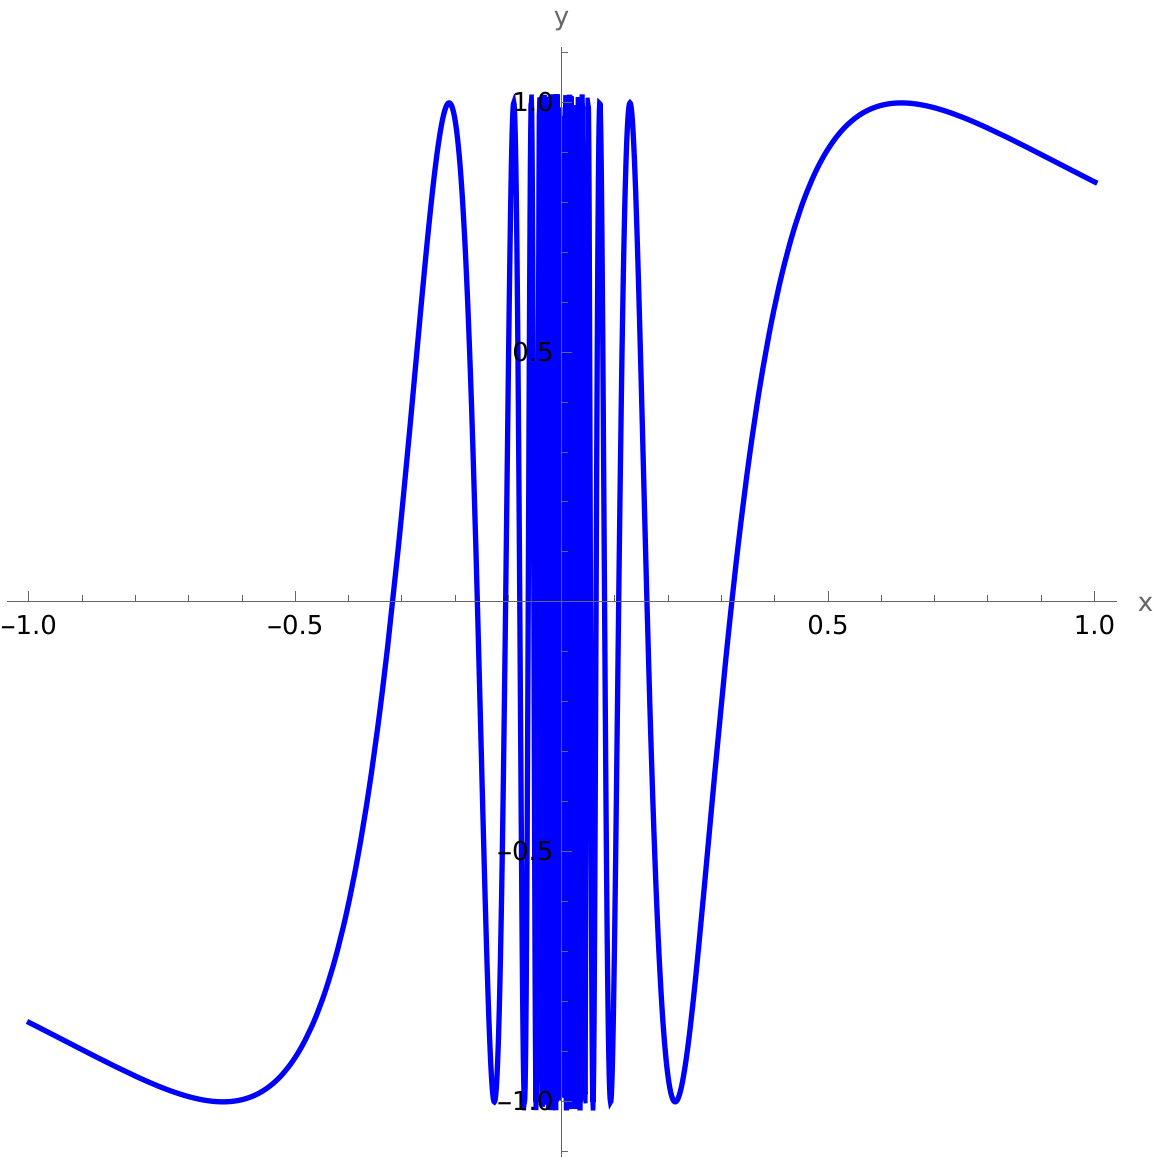
\includegraphics[width=0.4\linewidth]{sin1x.png}
		\caption{$f(x) = \sin(1/x)$}
		
	\end{figure}
\end{frame}


\begin{frame}
	\frametitle{$f(x) = \sin\left(\frac{1}{x}\right)$ 在 $x=0$ 处的不收敛性}
	
	考虑函数 $f(x) = \sin\left(\frac{1}{x}\right)$ 在 $x=0$ 处的极限. 
	
	\pause
	
	\textbf{定理: } 对于函数 $f(x) = \sin\left(\frac{1}{x}\right)$, 当 $x$ 趋近于零时, 极限不存在. 
	
	\pause
	
	\textbf{证明: } 
	我们可以通过构造两个不同的数列来证明这一点. 
	
	\pause
	
	\begin{itemize}
		
		\item 首先, 考虑数列 $\{x_n\} = \frac{1}{n\pi}$, 其中 $n$ 是正整数. 
		      
		      \pause
		      \begin{itemize}
		      	\item 当 $n$ 趋近于正无穷时, $x_n$ 趋近于零. 此时, $f(x_n) = \sin(n\pi) = 0$. 
		      	      
		      	      \pause
		      	      
		      	\item 因此, $\lim_{n \to \infty} f(x_n) = 0$. 
		      \end{itemize}
		      \pause
		      
		\item 接下来, 考虑数列 $\{y_n\} = \frac{1}{(2n+1)\pi/2}$, 其中 $n$ 是非负整数. 
		      
		      \pause
		      \begin{itemize}
		      	\item 当 $n$ 趋近于正无穷时, $y_n$ 趋近于零. 此时, $f(y_n) = \sin((2n+1)\pi/2) = (-1)^n$. 
		      	      
		      	      \pause
		      	      
		      	\item 因此, $\lim_{n \to \infty} f(y_n)$ 不存在. 
		      	      
		      	      
		      \end{itemize}
		      
		      \pause
		      
		\item 由于存在两个不同的数列 $\{x_n\}$ 和 $\{y_n\}$, 使得它们都趋近于零, 但对应的函数值却趋于不同的极限.
		      
	\end{itemize}
	\pause
	所以函数 $f(x) = \sin\left(\frac{1}{x}\right)$ 在 $x=0$ 处的极限不存在. 
\end{frame}

\begin{frame}
	\frametitle{符号函数在 $x=0$ 处的不收敛性}
	
	\begin{figure}
		\centering
		\begin{tikzpicture}[scale=2]
			% 坐标轴
			\draw[->] (-1.5, 0) -- (1.5, 0) node[right] {$x$};
			\draw[->] (0, -1.5) -- (0, 1.5) node[above] {$y$};
			% 函数图像
			\draw[domain=-1: 0, smooth, variable=\x, blue] plot ({\x}, {-1});
			\draw[domain=0: 1, smooth, variable=\x, blue] plot ({\x}, {1});
			% 坐标轴标签
			\foreach \x/\xtext in {-1/-1,  1/1}
			\draw (\x cm, 1pt) -- (\x cm, -1pt) node[anchor=north] {$\xtext$};
			\foreach \y/\ytext in {-1/-1,  1/1}
			\draw (1pt, \y cm) -- (-1pt, \y cm) node[anchor=east] {$\ytext$};
		\end{tikzpicture}
		\caption{$f(x) = \text{sgn}(x)$的函数图像}
	\end{figure}
	
\end{frame}

\begin{frame}
	\frametitle{符号函数在 $x=0$ 处的不收敛性}
	
	考虑符号函数 $f(x) = \text{sgn}(x)$ 在 $x=0$ 处的极限. 
	
	\pause
	
	\textbf{定理: } 对于符号函数 $f(x) = \text{sgn}(x)$, 当 $x$ 趋近于零时, 极限不存在. 
	
	\pause
	
	\textbf{证明: } 
	我们可以通过构造两个不同的数列来证明这一点. 
	
	\pause
	\begin{itemize}
		\item 首先, 考虑数列 $\{x_n\} = \frac{1}{n}$, 其中 $n$ 是正整数. 
		      
		      \pause
		      \begin{itemize}
		      	\item 当 $n$ 趋近于正无穷时, $x_n$ 趋近于零. 此时, $f(x_n) = \text{sgn}\left(\frac{1}{n}\right) = 1$. 
		      	      
		      	      \pause
		      	      
		      	\item 因此, $\lim_{n \to \infty} f(x_n) = 1$. 
		      \end{itemize}
		      \pause
		      
		\item 接下来, 考虑数列 $\{y_n\} = -\frac{1}{n}$, 其中 $n$ 是正整数. 
		      \begin{itemize}
		      	\pause
		      	
		      	\item 当 $n$ 趋近于正无穷时, $y_n$ 趋近于零. 此时, $f(y_n) = \text{sgn}\left(-\frac{1}{n}\right) = -1$. 
		      	      
		      	      \pause
		      	      
		      	\item 因此, $\lim_{n \to \infty} f(y_n) = -1$. 
		      	      
		      \end{itemize}
		      
		      \pause
		      
		\item 由于存在两个不同的数列 $\{x_n\}$ 和 $\{y_n\}$, 使得它们都趋近于零, 但对应的函数值却趋于不同的极限.
		      
	\end{itemize}
	
	\pause
	
	所以符号函数 $f(x) = \text{sgn}(x)$ 在 $x=0$ 处的极限不存在. 
	
\end{frame}

\subsection{函数极限的性质}
\begin{frame}
	\frametitle{函数极限的性质}
	
	\begin{itemize}
		\item<1-> \textbf{极限存在性}: 函数 $f(x)$ 在 $x=a$ 处有极限, 当且仅当左极限和右极限存在且相等. 
		\item<2-> \textbf{极限唯一性}: 如果函数 $f(x)$ 在 $x=a$ 处有极限, 则该极限是唯一的. 
		\item<3-> \textbf{局部有界性}: 如果函数 $f(x)$ 在 $x=a$ 处有极限, 则存在一个邻域 $N(a)$, 在该邻域内函数 $f(x)$ 是有界的. 
		\item<4-> \textbf{局部保号性}: 如果函数 $f(x)$ 在 $x=a$ 处有极限且不为零, 则存在一个邻域 $N(a)$, 在该邻域内函数 $f(x)$ 保持与极限符号相同. 
		\item<5-> \textbf{函数极限的四则运算}: 设函数 $f(x)$ 和 $g(x)$ 在 $x=a$ 处有极限, 则以下极限也成立: 
		\begin{itemize}
			\item $(f+g)(x)$ 的极限等于 $f(x)$ 和 $g(x)$ 的极限之和. 
			\item $(f-g)(x)$ 的极限等于 $f(x)$ 和 $g(x)$ 的极限之差. 
			\item $(f \cdot g)(x)$ 的极限等于 $f(x)$ 和 $g(x)$ 的极限之积. 
			\item $\left(\frac{f}{g}\right)(x)$ 的极限等于 $f(x)$ 和 $g(x)$ 的极限之商(假设 $g(x) \neq 0$). 
		\end{itemize}
	\end{itemize}
	
\end{frame}

% Thank you page
\beamertemplateshadingbackground{structure.fg!90}{structure.fg}
\begin{frame}[plain]
	\vfill
	\centering
	{
		\centering \Huge \color{white} Thank you for your attention!\\
		Questions?\\[10pt]Homeworks:  page 36:  20,  22,  27,  30; page 78:  3
		  
	}
	\vfill
\end{frame}


\end{document}

